\chapter{Introduction}
\addcontentsline{toc}{chapter}{Introduction}
\label{chpt:intro}
%Oli added this

\epigraph{The purpose of computing is insight, not numbers}{\textit{Richard Hamming, Numerical Methods for Scientists and Engineers}}

%\addcontentsline{toc}{chapter}{\color{green}Introduction}

%\epigraph{[Quantum computation] does not merely make computer science
%a branch of physics. \\ It also makes part of experimental physics into a %branch of computer science.}{\\ David Deutsch \\ Quantum theory, the %Church-Turing principle, and the universal quantum computer}

\subsection{Motivation for this guide/ the need for quantum programmers}

Quantum mechanics is one of the most well-tested theories in existence. It is also one of the most unintuitive, revealing aspects of nature at nanoscopic scales which are incompatible of our a human's experience of the world. 

There are two main facets which differentiate quantum from classical theory. The first is the quantisation of properties of a particle such as charge, angular momentum, and energy, from which the field derives its name. This feature has already changed the world substantially over the course of the last 70 years. In addition to technologies such as the laser and magnetic resonant imaging (MRI) \cite{ioplasers, odaibo2012quantumMRI}, perhaps the greatest impact has been made through the manipulation of semiconductor materials. Since the invention of the first transistor in 1947 \cite{Bardeen1948}, semiconductor technology has laid the groundwork for scalable computing, bringing us into the the current information age.

We are reaching a critical time in the conventional silicon industry. The famous `Moore's law', hypothesised in its current form in 1975, stated that the number of transistors per square inch would double every two years. This rule of thumb models the exponential scaling which computing power has followed since its conception incredibly well, as seen in \autoref{fig:Moore's_Law}. This was driven predominantly by the cost and power consumption per transistor going down as feature sizes decreased \cite{MooresLawEconomist}.  However, now increasingly small feature sizes have resulted in energy efficiencies and profitability are starting to plateau, while technical issues continue to increase. Some of these issues are in part due to quantum effects such as `tunnelling', where an electron is able to access regions in space where, classically, it would have insufficient energy to reach.  

\begin{figure}[!ht]
	\centering
	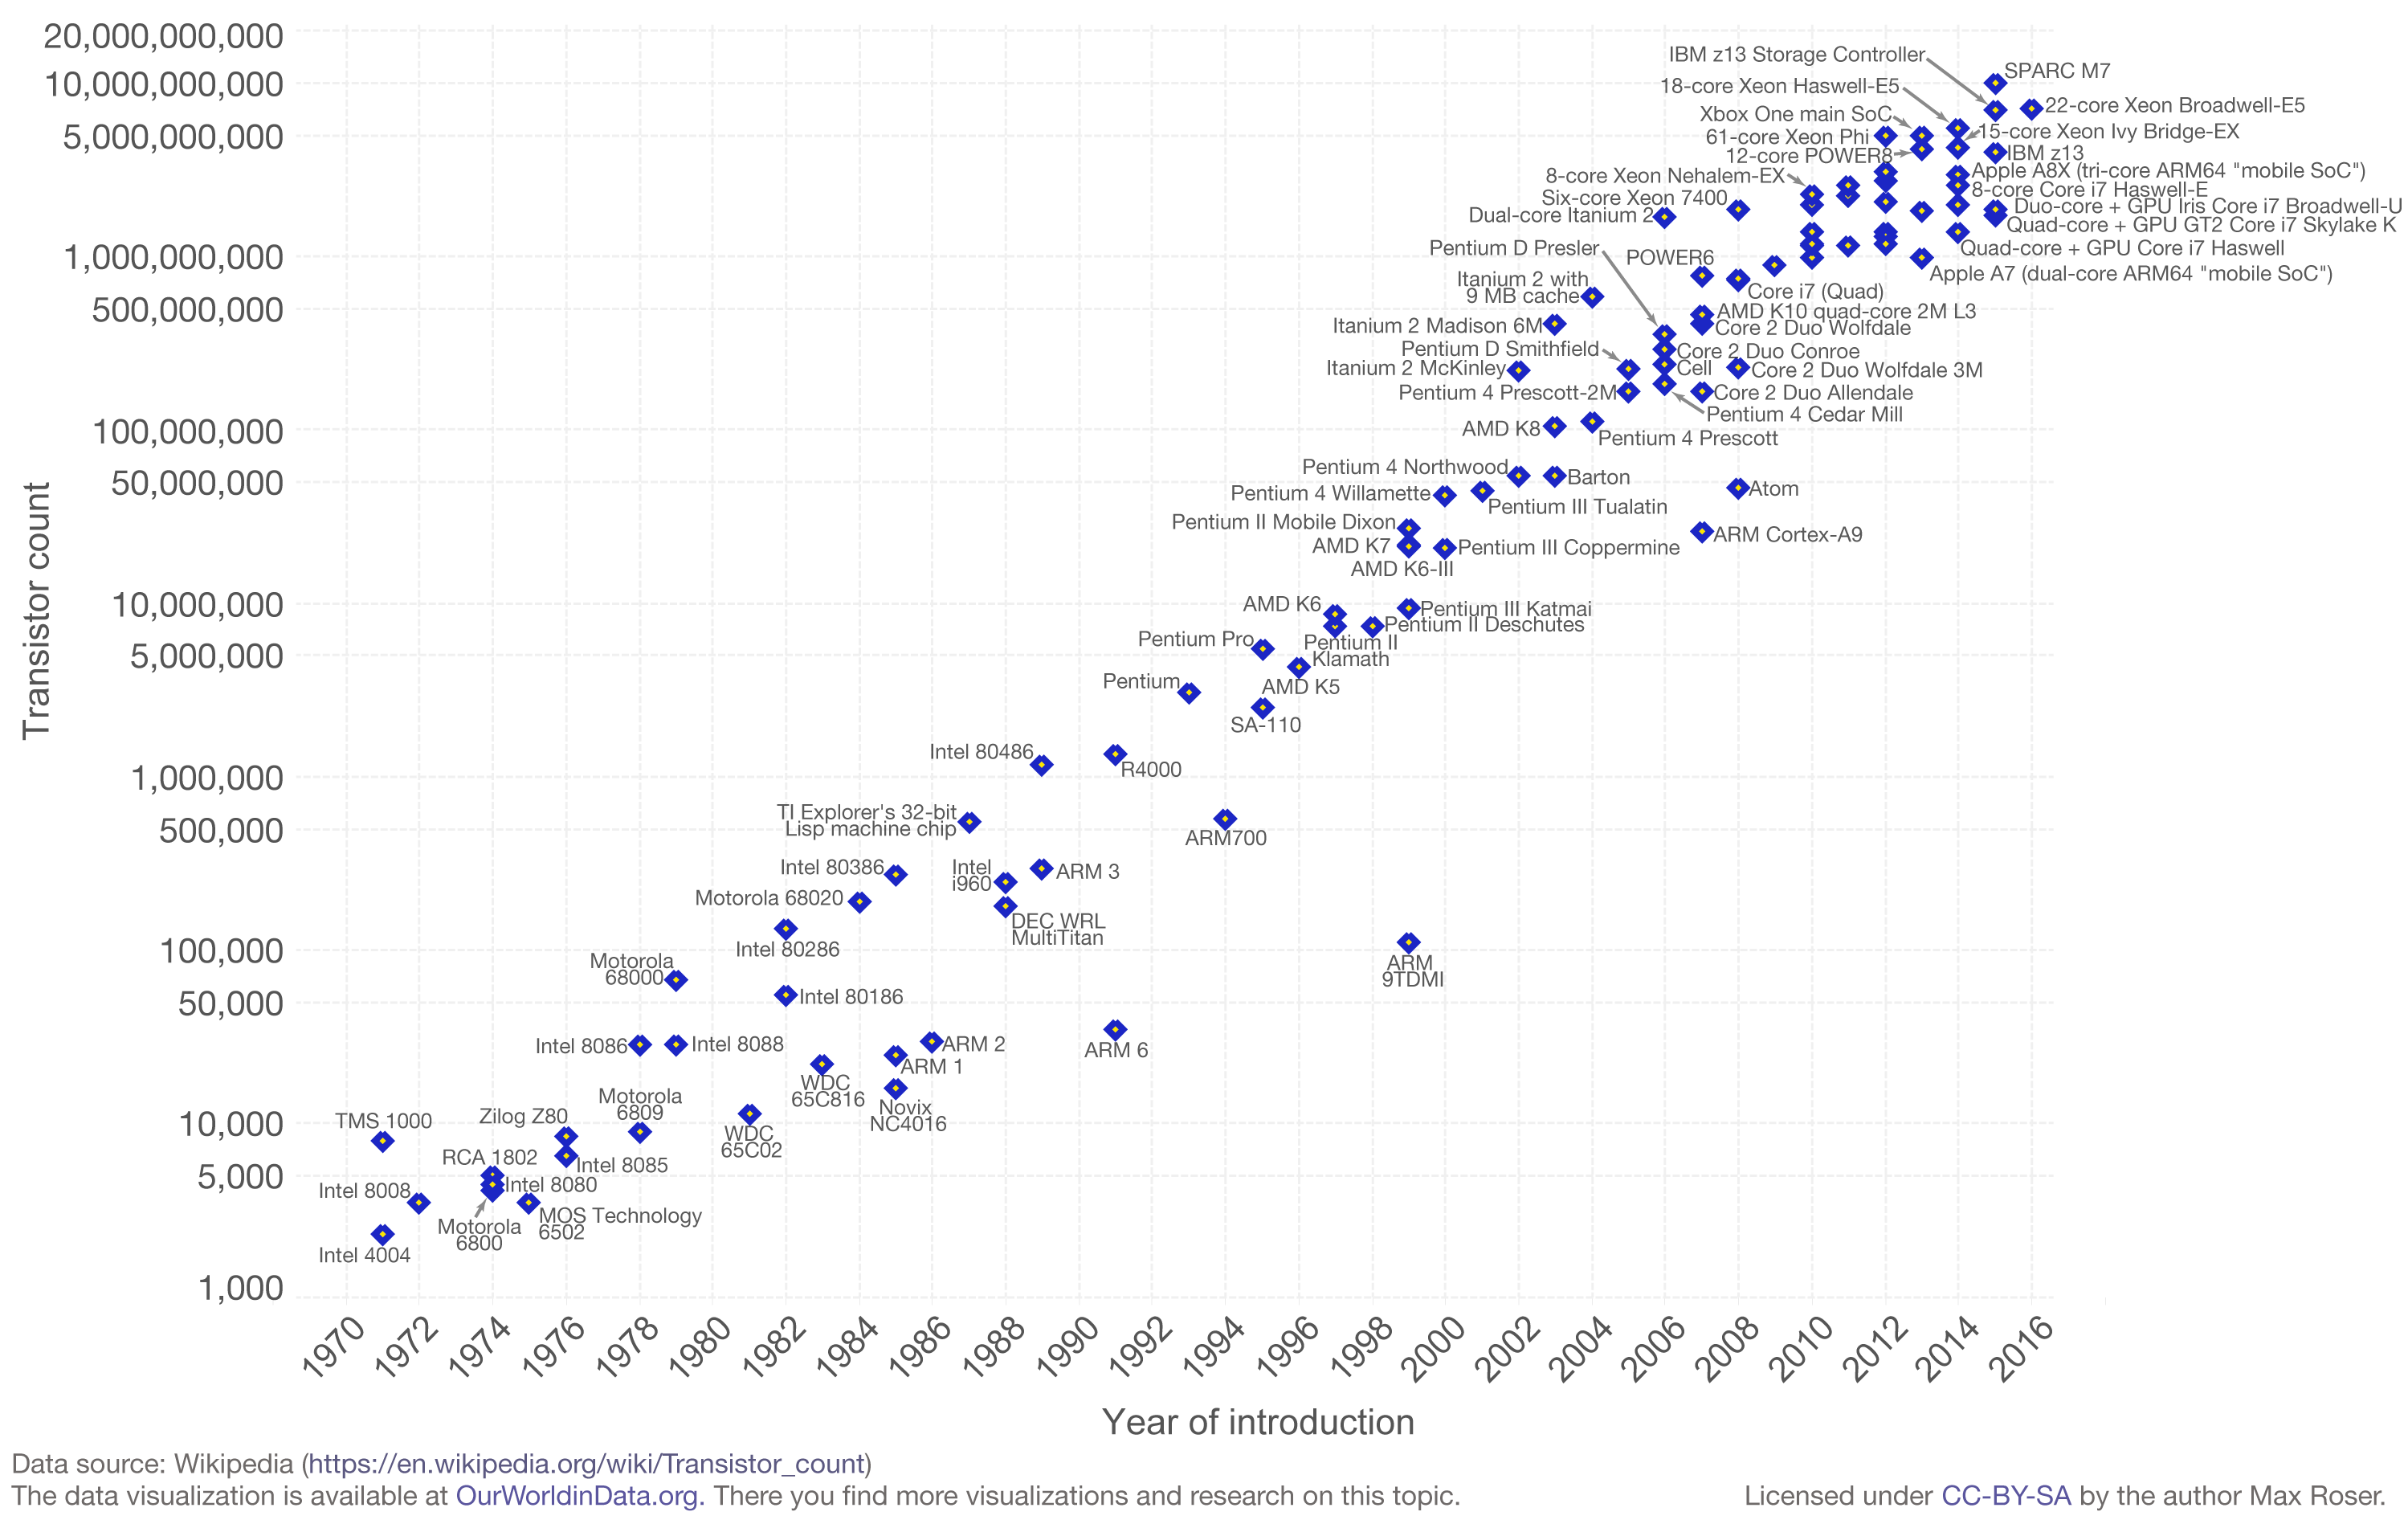
\includegraphics[width = \linewidth]{Moores_Law.png}
	\caption{Chart showing Moore's law, with a logarithmic increase in transistor 	count on each chip from 1970-2016.}
	\label{fig:Moore's_Law}
\end{figure}

This example of tunnelling is related to the so-called `wave-particle duality' - this is the second key feature of quantum mechanics. The distinction between waves and particles, whose behaviour is well established in classical physics, becomes blurred. Every object in the universe, depending on their energy and confinement, will display both of these aspects to some degree. 

The tantalising promise of quantum computing is hidden in this property. Particles such as electrons, which have comprised the backbone of electricity and classical information for the past century, have the ability to behave in a wave-like manner: they could contain not just the binary bit choices of 0 or 1, but some form of `superposition' of the two, giving many more possible values which can be processed. Currently for computationally difficult tasks supercomputers must be used, which require massive amounts of space and are costly to build and run. The current state of the art is the Summit supercomputer which is shown in figure  \autoref{fig:Summit} with 200 petaflops of computing power. With an exponential scaling in computational power, quantum computers are capable of performing tasks with fewer resources compared to classical \footnote{A classic example of the power of exponential scaling is given by the legend of a vizier who presented a gift to his King. The king asked what he wanted in return, and the vizier replied that he wanted rice. Precisely, he wanted one grain of rice on the first square of the chessboard, two grains of rice on the second, four grains on the third, and so on, doubling on each square. This bankrupts the king, who has to find $2^{63}$ grains of rice for the last square alone. This is $\sim 100$ times greater than the \emph{current} global annual food production (at $\sim 10^{12}$kg \cite{Globalfoodproduction}).}. Thus adding a single extra qubit could double the computing power. Combined with entanglement to allow our qubits to influence each other in these superposition states, we can harness a form of parallelism that results from the wave-like nature of controlled particles. 

While in general it is doubtful that a quantum computer will be universally  `faster' than a classical computer, and is much harder to engineer, these combined features of superposition and entanglement give quantum computers significant potential to outperform conventional computers at certain tasks. At the point when quantum computers are able to outperform classical supercomputers at a task, the so-called `quantum supremacy' will have been achieved \cite{Preskill2012}. 

% are we mentioning that we can simulate around 50-qubit Q computer with classical computers?

% Further references on Q supremacy. First time defined \cite{Preskill2012}, recently proposed algorithm \cite{QKitchenSinks2018}, theoretical work on the amount of qubits needed for it \cite{Harrow2018}, the article suggesting supremacy with Boson sampling is far away \cite{BSsupremacy2017}.

These tasks range from aiding the fields of medicine, chemistry and materials with applications including creating more powerful simulations\footnote{This application - the simulation of large, complex many body systems - was in fact one of the very first motivators for the development of quantum computers, most famously by Richard Feynman \cite{Feynman1982simulating}.}\cite{Georgescu2014Sim}; providing possible speedups for AI and machine learning \cite{Biamonte2017QML}; assisting with modelling complex logistics problems; and improving financial models \cite{Schaden2002quantumfinance}.

However, achieving this potential does not come without significant engineering difficulties. Readout or detection of the information in the qubit (measuring it) removes the quantum aspect of the information contained within, resulting in it reverting to the classical bit values with differing probabilities. This probabilistic nature is a fundamental (and irremovable) part of quantum theory. Furthermore, the technology is still young and undeveloped. On the hardware side, D-wave has many `quantum annealers' which can solve specific problems using quantum tunnelling, but the race to build a universal quantum computer is in an early stage. Academic institutions, large corporations (including Google \cite{googleqai, bristlecone}, IBM, \cite{ibmqweb} and Intel \cite{intelqcomp}) and smaller start-ups (Rigetti \cite{rigettihome}, Xanadu \cite{Xanadu}) alike have invested heavily in hardware. There are a wide range of platforms and architectures, including but not limited to superconducting qubits \cite{bristlecone}, ion traps \cite{steane1997ionTrap}, quantum dots \cite{loss1998quantumdots}, spin qubits in silicon \cite{intelSCspinqubits}, and silicon photonics \cite{RudolphSiliconPhotonicsQC}. 

\begin{figure}
    \centering
    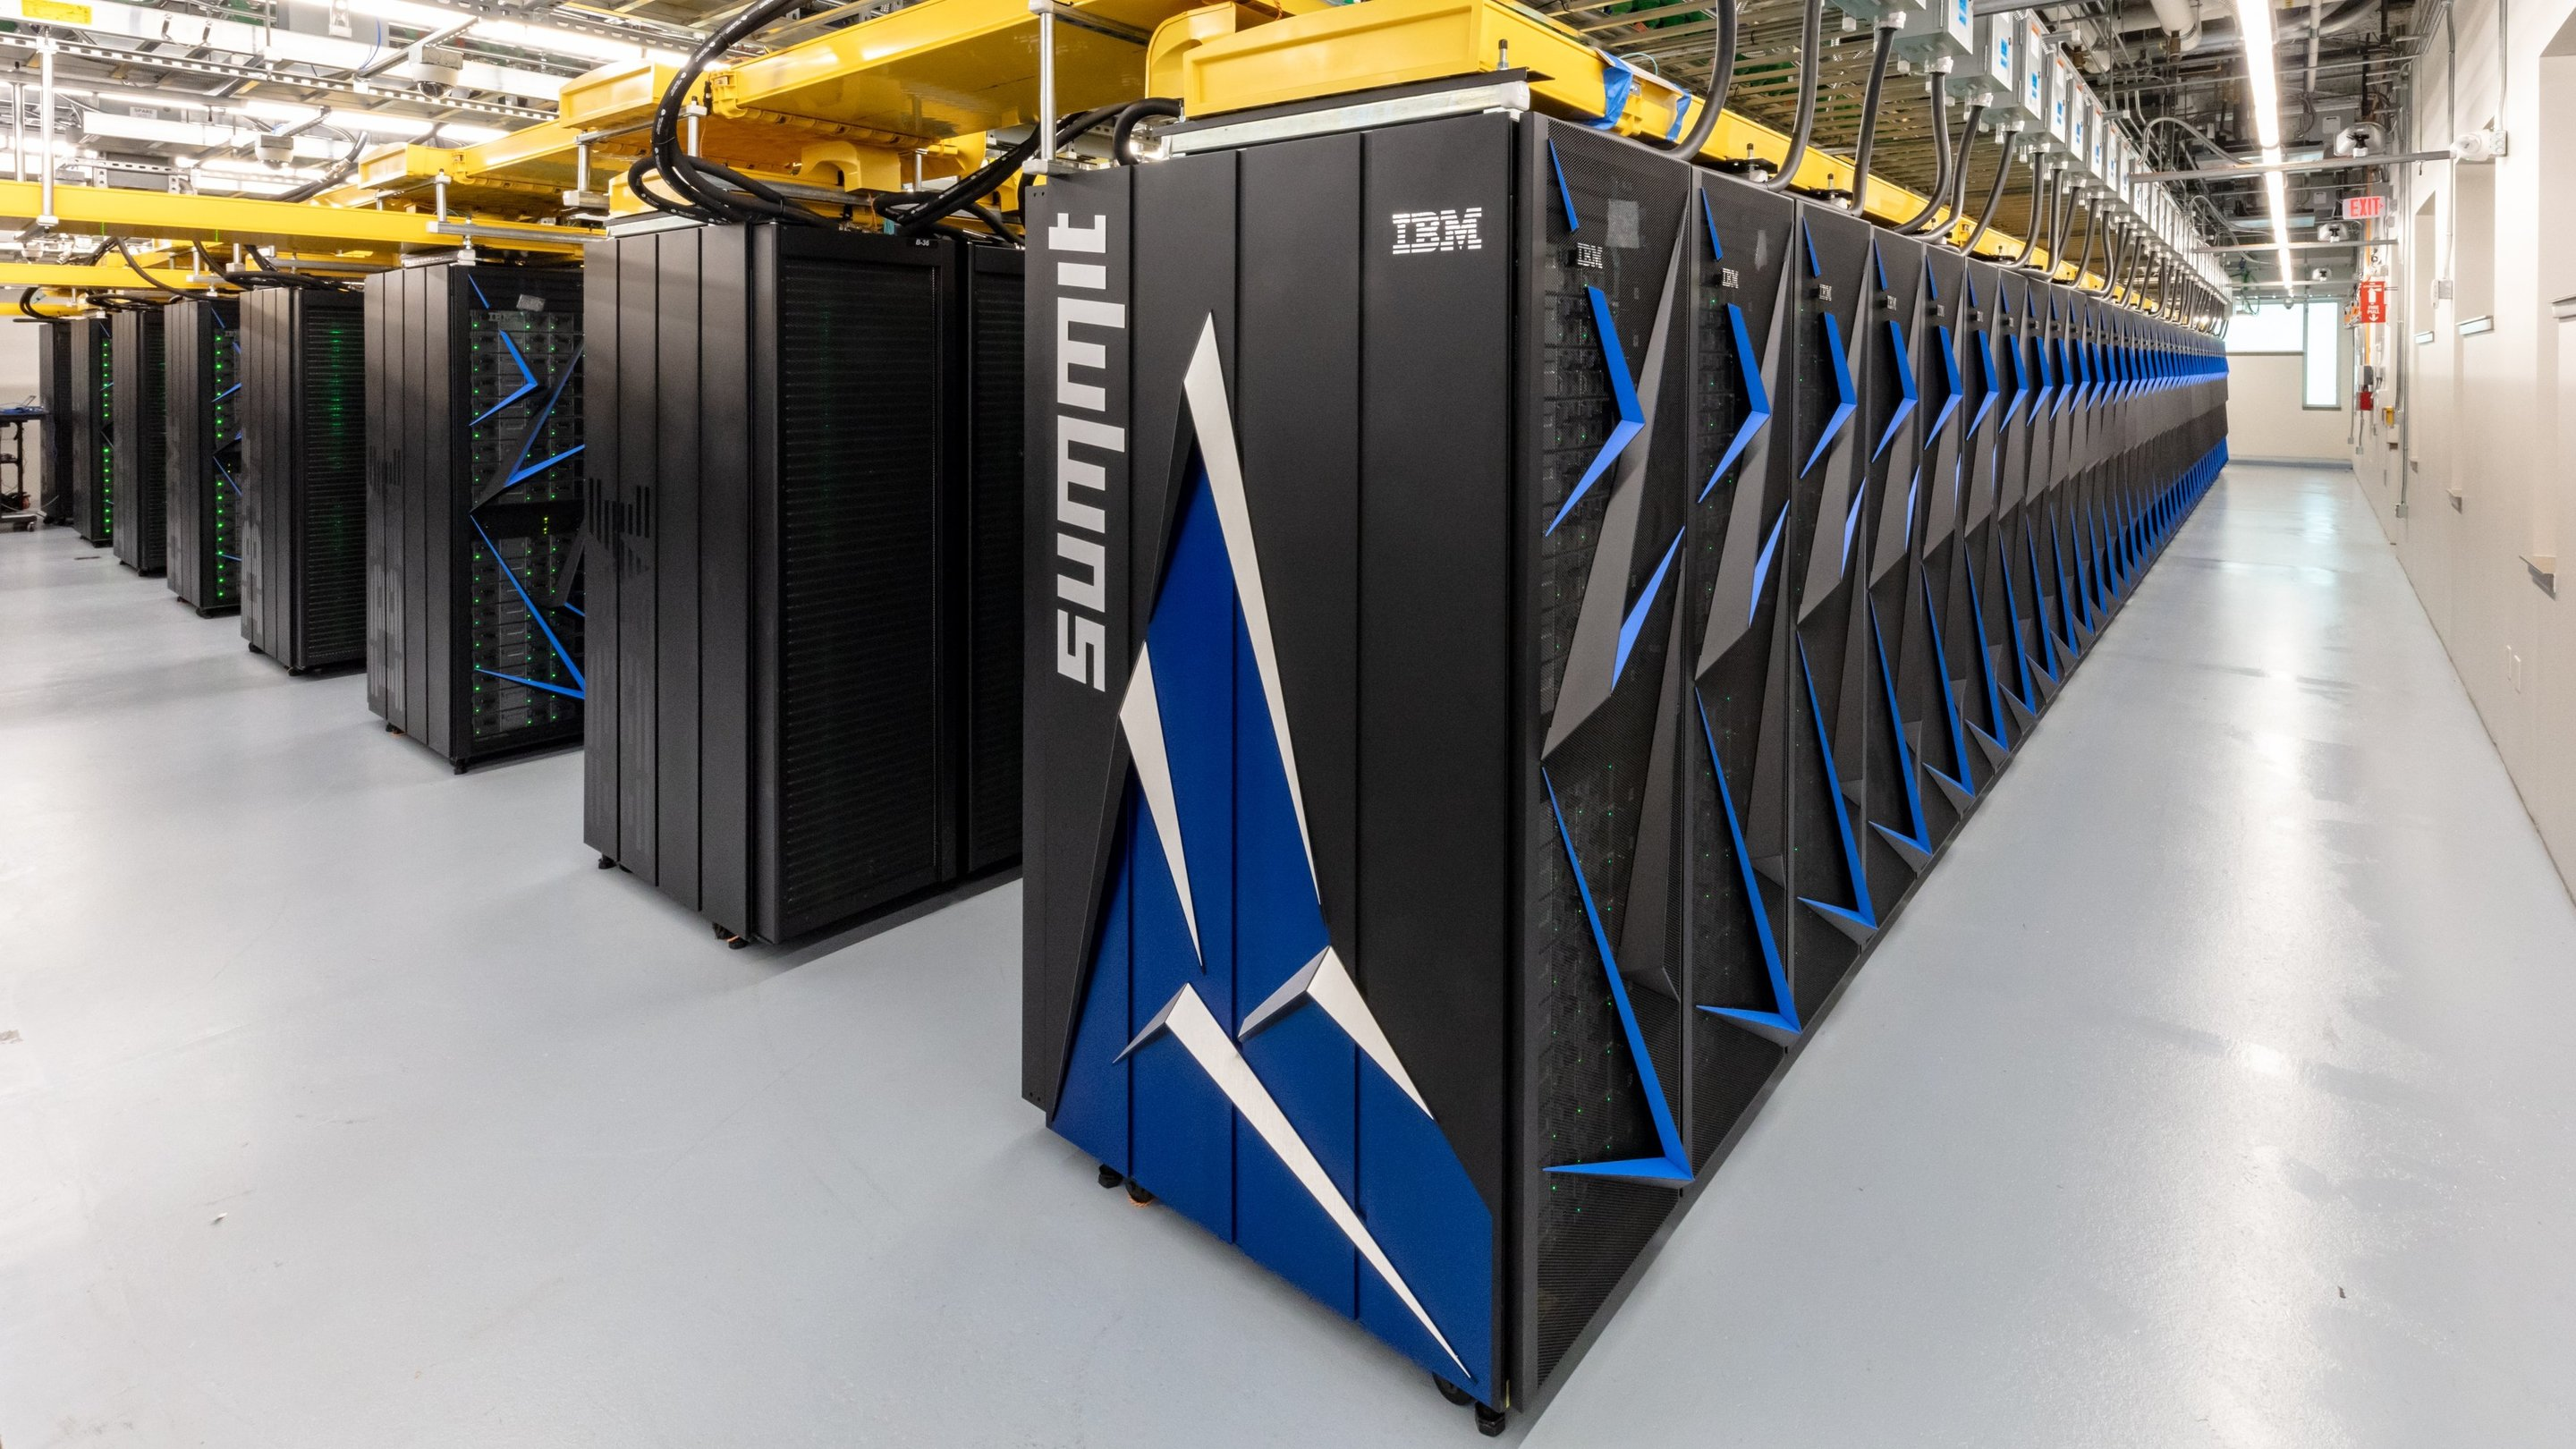
\includegraphics[width=\linewidth]{figures/SummitSC.jpg}
    \caption{The summit supercomputer, currently set to be the worlds fastest supercomputer, taking up the area of two tennis courts. \cite{SummitSC}}
    \label{fig:Summit}
\end{figure}

One area that remains comparatively underdeveloped is software. Algorithms exist for many of the applications above, but there may be many more as yet undiscovered. Furthermore, it will be crucial to provide the missing link between theoretical algorithm and their implementation on a quantum computer. Ideally `quantum' programming should adopt many of the features of its classical counterpart: it should be usable by any person without understanding the details of the hardware being used, while allowing access to the fundamental workings of the computer. However, all programming languages will have to trade off these two features to some degree. Finally it is required to translate the input of the user into a set of instructions that the computer can follow efficiently. This step is called compilation and is crucial to the ability to use computers.

This area has recieved significant attention recently, with a slew of documents addressing the issue of quantum software implementations  \cite{AlamosIBM2018, Xanadu2018, DK2018, DKBlog, RL2018, JW2018}. However, many of these documents focussed on one or two languages. In this guide, we intend to keep a broad overview of the current state of the languages out there. Furthermore, in the manner of conventional programming guides we provide worked examples and problems to aid newcomers to the field. 

%%%%%%%%%%%%%%%
\begin{comment}

There are alraedy several quantum programming languages in place, in this guide we are going to address pyquil by, QISKit by IBM, project Q and Q\#

also citing benchmarking \cite{JW2018}. Our guide is similar to \cite{RL2018} as in we are going to be comparing specific algorithm with different languages, the differences are this and that also all code in jupyter notebooks.

More resources for each programming language

Forest more Resources. pyQUIL other guides and resources. There are already programming guides addressing the use of pyQuil \cite{DK2018} and his blog \cite{DKBlog}.

QISKit more resoruces  \cite{IBM2018}.  \cite{RL2018}. 

Project Q more resources  \cite{RL2018}. 

Q\# more resources (ADD REFERENCES FOR OTHER GUIDES HERE)

REFERENCES for further languages compile this which we briefly describe at the end. \cite{Xanadu2018} \cite{IonQ}

\end{comment}
%%%%%%%%%%%%%


Over the next few years and decades quantum computing is likely to become a reality, eventually becoming accessible to people from a range of disciplines via cloud services. It will be crucial when this becomes the case that people are able to understand how to use these machines in order to harness their applicability to the areas of mathematics, computer science, chemistry and finance. This guide is designed to be an introduction to the science of quantum computers and the current state of the field. Initially we explain in-depth the working principles behind quantum computers and their differences to classical computers in \autoref{chpt:background}, and then introduce some of the current programming languages in We examine the programming languages that will be able to interface between the algorithms and the quantum computer in \autoref{chpt:quantumsoftware}. We go on to discuss a selection of algorithms and their applications in \autoref{chpt:algorithmsandapplications}.  

 Since in the short-term, quantum computers are likely to be noisy, error-prone and limited in scale, we discuss how they can be used in this regime in \autoref{chpt:shortqcomp}. While the long term software implementations are discussed in \autoref{chpt:programming}. Then we go on to consider and hardware-specific implementations and hardware/software architectures in detail in \autoref{chpt:implementations}. 

A more complete description of quantum mechanics is given in \autoref{chpt:advancedtopics} for any interested party. 
